\documentclass[]{article}
\usepackage{lmodern}
\usepackage{amssymb,amsmath}
\usepackage{ifxetex,ifluatex}
\usepackage{fixltx2e} % provides \textsubscript
\ifnum 0\ifxetex 1\fi\ifluatex 1\fi=0 % if pdftex
  \usepackage[T1]{fontenc}
  \usepackage[utf8]{inputenc}
\else % if luatex or xelatex
  \ifxetex
    \usepackage{mathspec}
  \else
    \usepackage{fontspec}
  \fi
  \defaultfontfeatures{Ligatures=TeX,Scale=MatchLowercase}
\fi
% use upquote if available, for straight quotes in verbatim environments
\IfFileExists{upquote.sty}{\usepackage{upquote}}{}
% use microtype if available
\IfFileExists{microtype.sty}{%
\usepackage{microtype}
\UseMicrotypeSet[protrusion]{basicmath} % disable protrusion for tt fonts
}{}
\usepackage[margin=1in]{geometry}
\usepackage{hyperref}
\hypersetup{unicode=true,
            pdftitle={narrativa\_tesis},
            pdfborder={0 0 0},
            breaklinks=true}
\urlstyle{same}  % don't use monospace font for urls
\usepackage{graphicx,grffile}
\makeatletter
\def\maxwidth{\ifdim\Gin@nat@width>\linewidth\linewidth\else\Gin@nat@width\fi}
\def\maxheight{\ifdim\Gin@nat@height>\textheight\textheight\else\Gin@nat@height\fi}
\makeatother
% Scale images if necessary, so that they will not overflow the page
% margins by default, and it is still possible to overwrite the defaults
% using explicit options in \includegraphics[width, height, ...]{}
\setkeys{Gin}{width=\maxwidth,height=\maxheight,keepaspectratio}
\IfFileExists{parskip.sty}{%
\usepackage{parskip}
}{% else
\setlength{\parindent}{0pt}
\setlength{\parskip}{6pt plus 2pt minus 1pt}
}
\setlength{\emergencystretch}{3em}  % prevent overfull lines
\providecommand{\tightlist}{%
  \setlength{\itemsep}{0pt}\setlength{\parskip}{0pt}}
\setcounter{secnumdepth}{0}
% Redefines (sub)paragraphs to behave more like sections
\ifx\paragraph\undefined\else
\let\oldparagraph\paragraph
\renewcommand{\paragraph}[1]{\oldparagraph{#1}\mbox{}}
\fi
\ifx\subparagraph\undefined\else
\let\oldsubparagraph\subparagraph
\renewcommand{\subparagraph}[1]{\oldsubparagraph{#1}\mbox{}}
\fi

%%% Use protect on footnotes to avoid problems with footnotes in titles
\let\rmarkdownfootnote\footnote%
\def\footnote{\protect\rmarkdownfootnote}

%%% Change title format to be more compact
\usepackage{titling}

% Create subtitle command for use in maketitle
\newcommand{\subtitle}[1]{
  \posttitle{
    \begin{center}\large#1\end{center}
    }
}

\setlength{\droptitle}{-2em}
  \title{narrativa\_tesis}
  \pretitle{\vspace{\droptitle}\centering\huge}
  \posttitle{\par}
  \author{}
  \preauthor{}\postauthor{}
  \date{}
  \predate{}\postdate{}


\begin{document}
\maketitle

\section{Introducción}\label{introduccion}

\$

\begin{footnotesize}
In biology, phylogenetics is the study of the evolutionary history and relationships among individuals or groups of organisms (e.g. species, or populations). These relationships are discovered through phylogenetic inference methods that evaluate observed heritable traits, such as DNA sequences or morphology under a model of evolution of these traits. The result of these analyses is a phylogeny (also known as a phylogenetic tree) – a diagrammatic hypothesis about the history of the evolutionary relationships of a group of organisms. Phylogenetic analyses have become central to understanding biodiversity, evolution, ecology, and genomes.
\end{footnotesize}

\$

De forma puntual el análisis filogenético tiene como objetivos
esenciales

\begin{itemize}
\item
  Encontrar vínculos evolutivos entre organismos, al analizar los
  cambios en los diferentes organismos durante la evolución.
\item
  Encontrar relaciones entre ancestros y sus descendientes, al analizar
  familias de secuencias
\item
  Estimar el tiempo de divergencia dentro de un grupo de organismos que
  comparten el mismo ancestro
\end{itemize}

Desde un punto de vista operacional, el análisis filogénetico tiene dos
componentes: La inferencia filogenética (o construcción de árboles) y la
aplicación de estas filogenias para entender la evolución de los
organismos y sus características.

La forma más común (y natural) de representar las relaciones evolutivas
entre un grupo de organismos es un \emph{árbol filogenético}. Este puede
ser de distinta configuración dependiendo qué se desea comunicar

\documentclass{article}
 \usepackage{graphicx}
 

\begin{document}
   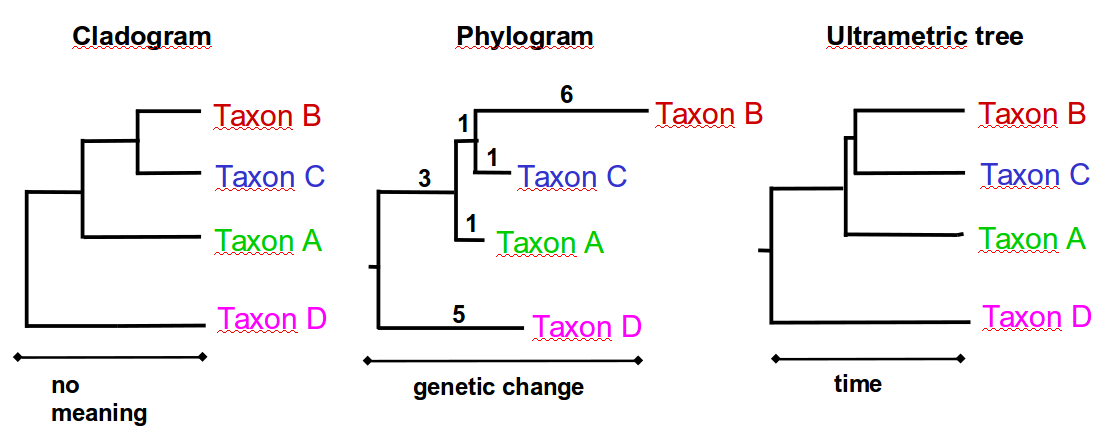
\includegraphics[width=0.5\textwidth]{treetypes.png}
 \end{document}


# Especificación del Problema

Se desea desarrollar o aplicar un algoritmo para que dada una secuencia de ADN, se clasifiqué de forma precisa* el taxa al que pertenece. 

Existen varios supuestos que son necesarios probar, el taxa que se desea estimar tiene una relación directa con la precisión esperada. En particular, a menudo las secuencias de ADN son más similares cuando los organismos son relativamente cercanos en términos evolutivos, por lo que la precisión será menor mientras el taxa a clasificar es más específico. 

Por otro lado es importante tener en cuenta que se debe elegir regiones del ADN que vayan acorde a la especifidad del taxa a clasificar. Es decir las cadenas de ADN a menudo son regiones específicas del genoma que son extraídas con base en parámetros de extracción y secuenciación. 

Por último, la cantidad de datos disponibles en las bases de datos públicas para poder es crucial realizar un análisis que generalice de forma adecuada.  


# Métodos (Computational Phylogenetics)

El objetivo principal es aplicar algoritmos, métodos computacionales para el análisis filogenético. El objetivo principal es construir un arbol que represente las hipótesis sobre la evolución  de un conjunto de genes, especies o taxones.  

La construcción de los arboles requiere una medida de homología entre las características observadas (morfológicas o moleculares).

- Métodos de Distancia

- Metodos de Parsimonia

- Metodos de Máxima Verosimilitud

- Métodos Bayesianos

Todos estos métodos dependen de forma implícita o explícita de un modelo matemático que describe la evolución de las caracteristicas observadas. En particular el concepto de arbol se puede generalizar al concepto de red filogenética, usado para analizar transferencia horizontal de genes. 

Más en https://en.wikipedia.org/wiki/Computational_phylogenetics

# Data Gathering

Es necesario encontrar un conjunto de datos que sean adecuados para realizar el experimento, esto se realiza usualmente mediante *Homologous Sequences Search*, que realiza un query a las bases públicas de datos genéticos

- BlastP (aaquery/aadb)
- BlastX (ntquery/aadb) 
  - nr (Non redundant protein ncbi) (2017-03-06)
  - Swissprot from NCBI ftp site (2017-03-06)
  - Refseq proteins (2017-03-21)
  - PDB AA (2017-03-06)
  - Uniprot (2010-03-04)

- BlastN (ntquery/ntdb)
- TBlastN (aaquery/ntdb)
  - genbank NT (2017-03-03)



# Revisión de Literatura

On process ...\footnote{Extraído de algún curso de posgrado de Sistemática Molecular} 

*Felsenstein, J. 2004. Inferring Phylogenies. Sinauer Associates, Sunderland MA.*

Freeman, S., and Herron, J.C. 2001. Evolutionary Analysis, 2nd Edition. Prentice Hall, Upper Saddle River, NJ.

Hillis, D.M., Moritz, C., and Mable, B.K. 1996. Molecular Systematics, 2nd Edition. Sinauer Associates, Sunderland MA.

Lee, W.-H. 1997. Molecular Evolution. Sinauer Associates, Sunderland MA.

Page, R.D.M., and Holmes, E.C. 1998. Molecular Evolution, a Phylogenetic Approach. Blackwell Science, Oxford.

**Required Articles**

Baldauf SL (2003) The deep roots of eukaryotes. Science 300:1703-1706

Stewart CB (1993) The Powers and Pitfalls of Parsimony. Nature 361:603-607

Zuckerkandl, E., and L. Pauling. 1965. Molecules as documents of evolutionary history. J. Theoret. Biol. 8:357-366.

Delwiche, C. F. 2004. The genomic palimpsest: Genomics in evolution and ecology. Bioscience 54:991-1001.

```


\end{document}
